\section{Ejercicio 2}

\subsection{Descripción del problema}

\subsubsection{Enunciado Informal}

En este problema se nos presenta un conjunto de ciudades con rutas entre las mismas que van en una sola dirección. No necesariamente se puede llegar desde una ciudad a cualquier otra pero necesariamente toda ciudad debe tener al menos una ciudad a la que se pueda viajar.
Cada una de las rutas tiene un determinado costo para realizar el viaje. Se desea reducir el costo de viajar en todas las rutas por un costo fijo C (puede llevar a que el costo de viajar en una ruta sea negativo). Se desea hallar el maximo C tal que no hay una camino que empieze en una ciudad y vuelva a esa misma ciudad con un costo total negativo.  

\subsubsection{Enunciado Formal}

Se tiene un grafo dirigido que no tiene ningun vertice de grado 0. Cada una de las aristas tiene pero determinado. Se desde hallar el maximo C tal que se reduce el peso de todas las aristas por ese valor fijo C (puede pasar a haber aristas con peso negativo), tal que no pase a haber ningun ciclo con peso total negativo.

\subsubsection{Formato de entrada y salida}
La entrada esta conformada por:\\
una línea con 2 entero N  y M con la cantidad de ciudades y de de rutas respectivamente;\\
M lineas con enteros c1 y c2 que indican cuales ciudades comunica la ruta a describir en la linea, seguido de un entero positivo P indicando el costo de viajar por la misma.
\\
La salida es un único entero Solución con el máximo valor por el cual se pueden disminuir todos los peajes.

\subsubsection{Ejemplo con Solucion}
Ejemplo:un ejemplo en que no queda ningun elemento sin pintar\\
Entrada:\\
4 5\\
0 1 3\\
1 2 1\\
2 1 2\\
0 3 6\\
3 0 4\\
Salida:\\
2\\
Explicacion:\\
En este grafo se presentan 2 ciclos que son el que va a 3 en un proceso de ida y vuelta al cual se le podria restar hasta 5, y el otro ciclo es que va de 0-1-2-3-0, al cual se le puede restar 2 porque el costo total del viaje termina en 0 pero si le restar 3 terminaria en -3. Entonces únicamente se puede restar hasta 2. Cualquier otro ciclo que incluya que vuelva hasta el punto de origen y luego vuelva a viajar por otro recorrido no sirve porque literalmente serian 2 ciclos en 1 y su costo sería la suma de los 2 costos por lo que NO sería negativo al menos que uno de los 2 sea ya negativo.



\subsection{Explicación de la solución}

 Primero es importante notar que no puede pasar que no existan ciclos en el grafo ya que al tener al menos una arista saliendo de cada vertice si se va siguiendo un camino partiendo de una arista cualquiera, el camino nunca puede terminar en un punto muerto, por lo que necesariamente deberá formarse un ciclo. En conclusión todo arista debe pertenecer a al menos un ciclo. Por lo tanto si tuviera todas las aristas negativas tendríaa todos los caminos negativos y al menos uno de ellos sería un ciclo. Entonces ya se sabe que no se puede restar más que el peso de la arista de mayor peso. Hallar la arista de mayor peso es muy rapido ya que solo se debe recorrer todas una vez teniendo una complejidad final de \bigo(M)\\
Ahora ya establecido lo anterior, para resolver este problema es importante mecionar que el algoritmo de Belman-Ford \url{https://en.wikipedia.org/wiki/Bellman–Ford_algorithm} es capaz de identificar todos los ciclos negativos que involucren vertices que son alcanzables desde el vertice desde el que parte el algoritmo y el mismo tiene complejiiad en el peor caso de \bigo(A*M), donde A es la cantidad de vertices alcanzables desde el vertice del que se partió. Esto es util ya que si se logra partir el bellman ford desde un conjunto de vertices tales que se logre cubrir la totalidad de los vertices del grafo exactamente una vez entonces se tendría un algoritmo con complejidad total \bigo(N*M) capaz de identificar en cualquier grafo dirigido, la presencia de un ciclo negativo. Para hacer esto se hará que cada iteración de bellman ford guarda la lista de vértices que fueron alcanzados desde el vértice original (es decir los vértices tales que al final del bellman ford la distancia que tiene al vertice original sea menos que infinito) y si el vértice fue previamente vistitado en otra itreación de bellman ford se ingorarán todas las aristas que lo involucren. Esto permite que no se vuelvan a recorrer los ciclos partiendo desde un vértice que ya fue incluido (ya que hallar los caminos de A a B y de B a C va a incluir los caminos de B a C). Al hacer esto cada vértice a lo sumo será visitado una vez. Ademas para evitar correr N-1 pasos en cada Bellman ford se realizara una pequeñá modificacion por la cual se dejara de intentar actualizar las distancias cuando la cantidad de pasos que se realizo en el bellman ford supere la cantidad de vertices alcanzados (ya que no puede haber ningún camino mas largo que la cantidad de vertices del mismisimo conjunto de vertices alcanzables). Por lo tanto al final de esto se correr varios bellman ford intentando partir de todos los vertices sucesivamente (si ya fue incluido como parte de los visitable desde una anterior ese vertice será ignorado) de modo tal que se encontrarán todos los ciclos negativos sin necesidad de incluir ningún vertice en 2 bellman ford distinto. Por lo tanto este paso termino teniendo una complejidad de \bigo(N*M) como era buscado.\\
Ahora teniendo esto solo resta hacer una busqueda binaria donde se pruebe restar los distintos valores para restar (son menores o iguales a K por lo explicado al principio) y hallar el máximo valor de k tal que la combinación de Bellman-Ford no incluya ningun ciclo negativo. Por lo tanto al estar usando busqueda binaria solo se deben probar log(K) valores posibles para restar. Como tenemos que para cada valor a probar se necesita correr un algoritmo de complejidad \bigo(N*M) se tiene que la complejidad final sería \bigo(N*M*log(K)) lo cual es exactamente la complejidad pedida.\\


Para el pseudocodigo se utilizara una función que se encarga por su cuenta de hacer Bellman-Ford mientras que el codigo princial search solution se encargaria de hacer la busqueda binaria e ir haciendo los llamados a bellman ford . Ademas el vector edges tine tuplas que indicar los 2 vertices de la lista c1 c2 siendo c1 el de origen y c2 el de llegada. Mientras tanto el tercer elmento de la tupla es el peso de dicha arista.



	\algoritmo{searchsolution}{entero n,entero m, $vector<tupla<entero, entero,entero>> edges$}{entero}{\bigo($N*M*log(K)$)}{
	
\State Max $\gets$ 0 \comment \bigo($1$)	
\For {i $\gets edges[0],edges[1],...,edges[m-1]$} \comment se repite m veces
\State Max $\gets$ maximo(max,i[2]) \comment \bigo($1$)

\EndFor	

\If {$max=0$}  \comment \bigo($1$)
	\State devolver 0 \comment \bigo($1$)
\EndIf


\If {$max>0$}  \comment \bigo($1$)

\State $limiteizquierdo \gets -1$ \comment \bigo($1$)
\State $limitederecho \gets max+1$ \comment \bigo($1$)
\While {$limitederecho - limiteizquierdo > 1$} \comment se repite a lo sumo log(k) veces por ser una busqueda binaria)
	\State $medio \gets limiteizquierdo+ (limitederecho-limiteizquierdo)/2$ \comment \bigo($1$)
	\If {$bellmanford(n,m,edges,-medio)=true$} \bigo($n*m$)
		\State $limitederecho \gets medio$ \comment \bigo($1$)
	\EndIf
		\If {$bellmanford(n,m,edges,-medio)=false$} \bigo($n*m$)
		\State $limiteizquierdo \gets medio$ \comment \bigo($1$)
	\EndIf


\EndWhile
\State devolver limite izquierdo
\EndIf
	

 
}{\bigo(M)$+log(k)*2 $\bigo(N*M)}


\algoritmo{bellmanford}{entero n,entero m, $vector<tupla<entero, entero,entero>> edges$,entero modificador}{entero}{\bigo($N*M$)}{
	
	\State respuesta $gets$ FALSE
\State Crear visitado que es arreglo que indica si fue visitado el vertice. Empizan todos en no visitados 	
\For {i $\gets $ 0,1,...n-1} 

\If {$visitado[i]=FALSE$}  
\State visitado[i] $\gets$ TRUE
	\State Crear distancia que es arreglo que indica la distancia de cada vertice al vertice de origen i. Empizan todos en infinito 
	\State distancia[0] $\gets$ 0
	\State Ivertex $\gets$ 0
	\State limit $\gets$ 1
	\State distanceModifired $\gets$ TRUE
	\While {$distanceModified=TRUE \wedge Ivertex<limit$}
		\State distanceModified $\gets$ FALSE
		\For {edge $\gets$ edges[0],edges[1],...,edges[m-1] }
			\State edgeweight $\gets edge[2]+modificador$
			\State v1 $\gets edge[0]$
			\State v2 $\gets edge[1]$
		
			\If {$distancia[v1]\neq INFINITO \wedge distancia[v1]+edgeweight<distance[v2] \wedge visitado[i]=FALSE$}
			\State $limit \gets limit+1$
			\State $visitado[v2] \gets TRUE$
			\State $distancia[v2] \gets distancia[v1]+edgeweight$
			\State distanceModified $\gets TRUE$
			\EndIf
		\EndFor
	
		\State Ivertex $\gets$Ivertex+1
	\EndWhile	
	
	\If {Ivertex=limit}	
		\State respuesta $\gets$TRUE
	
	\EndIf
		
\EndIf


\EndFor	
\State devolver respuesta



	

 
}{}

\subsection{Experimentación}
Experimentación\\
 
Ejercicio 2:\\
 
La experimentación del ejercicio 2 se llevó a cabo generando instancias de test de distintas características. En particular, se deben notar algunas particularidades acerca de los grafos generados:\\
 

\begin{itemize}  
\item Cada grafo generado tiene k componentes conexas
\item Todas las componetnes conexas son componentes fuertemente conexas del grafo
\item Para fijar la cantidad de aristas en un grafo de variables componentes (fuertemente) conexas, se estableció la cantidad mínima de aristas para el grafo de mayor cantidad de componentes. Para cualquier otro grafo de menos componentes, la cantidad mínima de aristas es menor, con lo cual las aristas que restan requeridas para llegar al “m” fijado se redistribuyen entre las componentes restantes.
\item Para variar la densidad del grafo, la diferencia entre la máxima y mínima cantidad de aristas para una componente conexa se múltiplica por un modificador de densidad entre 0.0 y 1.0. La cantidad de aristas asignadas asignadas a la componente es esta más las mínimas necesarias para que sea fuertemente conexa.
\item Para la generación de aristas, en cada componente conexa se genera un ciclo (v1, v2), (v2, v3)...(vN, v1). El costo de este ciclo es de 0. Si la cantidad de aristas que se debiera tener la componente es mayor, entonces se toman todas las posibles aristas que se pueden agregar, se ordenan aleatoriamente en una secuencia, y se toma la cantidad de aristas restantes, con costo max(c) deseado. Con esto nos aseguramos que la búsqueda binaria llegue hasta el final (ya que de tomar cualquier c, el ciclo (v1, v2), (v2, v3)...(vN, v1) se torna negativo).
 

\end{itemize}

Dentro de las observaciones que podemos hacer acerca del algoritmo se encuentra una relacionada a la cantidad de componentes fuertemente conexas del grafo de entrada. En un análisis de tiempo de ejecución del algoritmo, se podría concluir que el mismo es independiente de las componentes conexas que tenga el grafo. Esto significa que dados un n, m y max(c) fijo, y variando la cantidad de componentes conexas, el tiempo de ejecución se mantiene igual. Observamos a continuación la distribución del tiempo en base a las variaciones en cantidad de componentes conexas. Para estas instancias se tomaron samples de hasta 200 componentes conexas en grafos de 600 nodos y 600 aristas con max(c) = 100.\\


\begin{figure}[!htb!]
	\begin{center}
		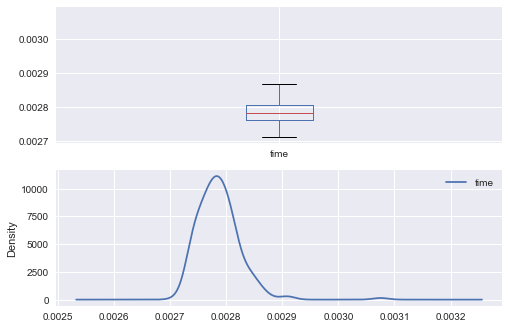
\includegraphics[width=300pt]{Imagenes/componentes_conexas.png}
		\caption{{\small \textit{componentes conexas}}}
	\end{center}
\end{figure}

Otra observación interesante tiene que ver con la tendencia de la complejidad algorítmica dependiendo de variaciones en la densidad del grafo. Para grafos de baja densidad la cantidad de aristas tiende a n, y para grafos de alta densidad, la cantidad de aristas se acerca a $n^{2}$. Si fijamos max(c) y variamos la densidad para observar estos cambios, podemos ver cómo varía la correlación entre estas complejidades. \\
A continuación mostramos tres gráficos: Una comparación entre los tiempos del algoritmo para densidad 0 y densidad 1, la correlación pearson entre $n^{2}$ y los tiempos de ejecución del algoritmo para grafos de baja densidad, y la correlación pearson entre $n^{3}$ y los tiempos de ejecución del algoritmo para grafos de alta densidad. En este caso se tomaron grafos de hasta 200 nodos.
\\
\begin{figure}[!htb!]
	\begin{center}
		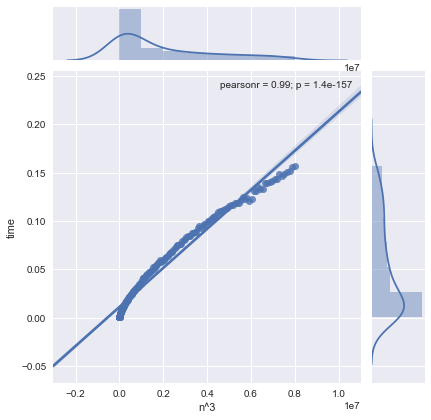
\includegraphics[width=200pt]{Imagenes/high_density_vs_n3.png}
		\caption{{\small \textit{alta densidad vs $n^{3}$}}}
	\end{center}
\end{figure}

\begin{figure}[!htb!]
	\begin{center}
		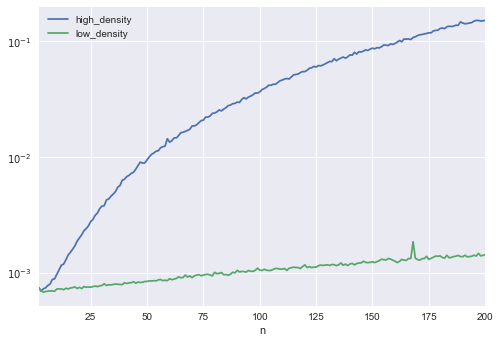
\includegraphics[width=200pt]{Imagenes/high_vs_low_density.png}
		\caption{{\small \textit{alta vs baja densidad}}}
	\end{center}
\end{figure}

\begin{figure}[!htb!]
	\begin{center}
		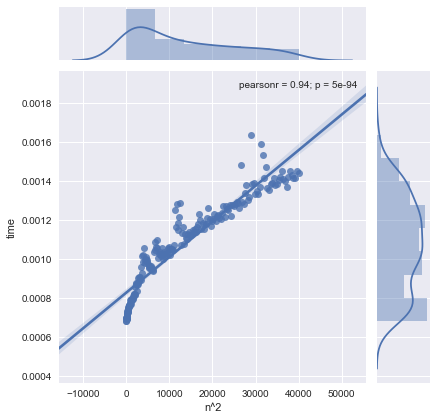
\includegraphics[width=200pt]{Imagenes/low_density_vs_n2.png}
		\caption{{\small \textit{baja densidad vs $n^{2}$}}}
	\end{center}
\end{figure}
\pagebreak




